\documentclass[12pt]{article}

\usepackage{float} % enable use of H for placing tables/figures %

\usepackage{array} % enable table columns with left, right, centre %
			       % alignment %
\newcolumntype{L}[1]{>{\raggedright\let\newline\\\arraybackslash\hspace{0pt}}m{#1}}
\newcolumntype{C}[1]{>{\centering\let\newline\\\arraybackslash\hspace{0pt}}m{#1}}
\newcolumntype{R}[1]{>{\raggedleft\let\newline\\\arraybackslash\hspace{0pt}}m{#1}}

\usepackage{textcomp}	% for enabling upquotes %
\usepackage[T1]{fontenc} % for having upquotes for double quote %
\usepackage{listings}   %for text/code commands%
\lstset{
    showstringspaces=false, % get rid of little space characters%
    upquote=true,           % change quotes to upquotes%
    language=bash,
    basicstyle=\footnotesize,
    numbers=left,           % add line numbers
    stepnumber=1,
    tabsize=1,
    breaklines=true,
    breakatwhitespace=false,
    literate={~} {$\sim$}{1} % add nice tilde symbol
}  

% set-up clickable links in pdf %
\usepackage{hyperref}
\hypersetup{
    colorlinks,
    citecolor=black,
    filecolor=black,
    linkcolor=blue,
    urlcolor=blue
}

\usepackage[margin=1.25in]{geometry} %make margins not gross%

\usepackage[labelfont={bf}]{caption} %make caption names bold%

\usepackage{graphicx}	%for pictures%
\graphicspath{ {pics/} }	%where my pictures are located relative to%
						%the folder where my main document is saved%

\def\changemargin#1#2{\list{}{\rightmargin#2\leftmargin#1}\item[]}
\let\endchangemargin=\endlist % enable margin changes for pages %

\title{Specific Information for HPC Resources and MD Simulation File Structures}
\author{Jennifer Garner}
\date{April 21st, 2017}


\begin{document}
\pagenumbering{arabic}
\maketitle
\newpage
\tableofcontents
\newpage

\section{Jen's Guide to the Terminal}

\quad\enskip\quad The linux terminal accepts bash commands for navigating file systems, moving and copying files between directories, editing files, accessing remote servers, and running programs (i.e. job submission). Some helpful terminal commands are: ls, pwd, cd, mkdir, cp, scp, mv, chmod, man, grep, awk, which, and ssh. These will be further explained. See Table \ref{big-table} for a summary on these commands.

\subsection{Navigating the Terminal}

\quad\enskip\quad When the terminal is opened, the user will most likely be in the home directory. This home directory is usually \textit{/home/username} - this string of text is called a path. The current path, which can be determined using the command \textit{pwd} or \textit{present working directory}, is the user's location on the computer, starting with the root directory (/). The terminal is case-sensitive, and requires the use of forward-slashes (/) to denote the end of each directory name. Commands are given after the prompt, which is usually the dollar sign (\$). 

\quad To determine what is in the home directory, the command is \textit{ls}. This command has optional arguments, which are denoted by a hyphen (-). Some common arguments are: \textit{-a} to display hidden files and directories, \textit{-l} to show more information on the contents of a directory, and \textit{-h} to give the file sizes in "human readable" format (i.e. using KB, MB, and GB designations as opposed to size in bytes). Hidden files and directories begin with a dot (.).

\begin{lstlisting}[numbers=none]
		username@pcname:~$ pwd
		/home/username		
		username@pcname:~$ ls
		Documents  Pictures  Templates Downloads  Music
		Public     Videos    Desktop
		username@pcname:~$ ls -l
		total 56
		drwxr-xr-x  2 ownername groupname 4096 Apr 17 14:54 Desktop
		drwxr-xr-x 11 ownername groupname 4096 Apr 18 15:12 Documents
		drwxrwxr-x  2 ownername groupname 4096 Apr 18 14:54 Downloads
		drwxr-xr-x  3 ownername groupname 4096 Aug 12  2016 Music
		drwxr-xr-x  5 ownername groupname 4096 Apr 17 12:09 Pictures
		drwxr-xr-x  2 ownername groupname 4096 Jul 25  2016 Public
		drwxr-xr-x  2 ownername groupname 4096 Jul 25  2016 Templates
		drwxr-xr-x  2 ownername groupname 4096 Sep 17  2016 Videos
\end{lstlisting}
\quad\enskip\quad The file system on linux can be thought of as a tree, where the root directory is the top of the tree and the subsequent directories are branches from that tree. To access the home directory from any location, use the command \textit{cd \$HOME}, where cd stands for \textit{change directory}. Note that after changing the directory to Documents, the length of the prompt increases to include the new path. The tilde key ($\sim$) can also be used to reference the home directory; \textit{$\sim$/Documents} is the same path as \textit{/home/username/Documents}.

\quad To go up one directory, the command is \textit{cd ../}. The current directory is usually denoted by \textit{./}; therefore, \textit{cd ./../} and \textit{cd ../} are the same command. When the \textit{cd} command is not preceded by a slash, the \textit{./} is implied. If the \textit{cd} command is used to try and access a file rather than a directory, the error "Not a directory" will appear. If the \textit{cd} command is used to try and access a directory that is not available (located somewhere else on the computer), the error "No such file or directory" will appear. A common error with file navigation is to try a command such as \textit{cd /Documents/}. This commmand will return the "No such file or directory error", because the initial forward slash (/) denotes the root directory, which does not contain a directory called Documents.

\begin{lstlisting}[numbers=none]
		username@pcname:~$ cd Documents/
		username@pcname:~/Documents$ pwd
		/home/username/Documents
		username@pcname:~/Documents$ cd ../
		username@pcname:~$ cd Documents/
		username@pcname:~/Documents$ cd $HOME
		username@pcname:~$ pwd
		/home/username
\end{lstlisting}
\quad\enskip\quad Some linux systems have colouring on the terminal to indicate the difference between a file (white/black, depending on terminal background colour), an executable file (one that can be run - green), a directory (blue), a linked file (cyan), a picture file (purple), and a compressed (zipped) file (red). If colouring is not enabled by default, the command \textit{ls $--$color=auto} can be used.

\quad Depeneding on the specific operating system (OS), copying and pasting files from the terminal may require the use of Ctrl-Shift-C and Ctrl-Shift-V instead of the usual Ctrl-C and Ctrl-V. 


\subsection{File Permissions}
\quad\enskip\quad Recall that executable files are different from regular text files. An executable file will have an `x' category when the ls -l command is used. The position of the x depends on who can execute the file (or which class - see table below). The three permissions that a class can have are: read (r), write (w), and execute (x). If permission is not given for a class, the hyphen will be present (-).

\begin{table}[H]
\centering
{\renewcommand{\arraystretch}{1.2}% for the vertical padding
\begin{tabular}{cccc|ccc|ccc}
 & \multicolumn{9}{|c}{Permissions by Class} \\
\cline{2-10}
Directory (d) & \multicolumn{9}{|c}{all (a)} \\
\cline{2-10}
Not a directory (-) & \multicolumn{3}{|c|}{user (u)} & \multicolumn{3}{c|}{group (g)} & \multicolumn{3}{c}{others (o)} \\
\hline
d & \multicolumn{1}{|c}{r} & w & x & r & w & x & r & w & x 
\end{tabular}
}
\end{table}
\quad For example, to change the regular file ex1.bash to an executable file, use the command \textit{chmod u+x ex1.bash}. This command makes the file executable (x) for the current user (u). To remove this same permission, the command \textit{chmod u-x ex1.bash} can be used. The current user can be determined by using the command \textit{echo \$USER}. The file can also be made executable for other classes, such as the group class and the others class, by specifying g or o respectively.

\begin{lstlisting}[numbers=none]
	username@pcname:~/examples$ ls -l
	total 16
	-rw-rw-r--  1 ownername groupname   33 Apr 21 17:12 exectuable.bash
	-rw-rw-r--  1 ownername groupname    0 Apr 21 17:12 textfile.txt
	drwxrwxr-x  2 ownername groupname 4096 Apr 24 10:19 example-directory/	
	username@pcname:~/examples$ chmod u+x exectuable.bash 
	username@pcname:~/examples$ ls -l
	total 4
	-rwxrw-r--  1 ownername groupname   33 Apr 21 17:12 exectuable.bash
	-rw-rw-r--  1 ownername groupname    0 Apr 21 17:12 textfile.txt
	drwxrwxr-x  2 ownername groupname 4096 Apr 24 10:19 example-directory/
\end{lstlisting}
\quad\enskip\quad Sudo is a group that have control over all files on a system.

\subsection{Aliases}

\quad\enskip\quad Sometimes a user will want to make "shortcuts" to their frequent commands. These shortcuts - called aliases - allow for short strings of text to be entered in place of longer commands. Aliases are stored in the user's home directory and are contained within hidden files. Using the command \textit{ls -a} from the home directory will determine the default alias files available. In Ubuntu, aliases can be stored within the file \textit{.bashrc}. However, it is recommended that the user make a new file, called \textit{.bash\_aliases}, for their personal commands. This file may already be present in the home directory.

\quad To start, open the .bashrc file from the home directory. You can use any text editor to do this, such as gedit, nano, vim, emacs, etc. For example, to open the file using gedit, the command would be \textit{gedit $\sim$/.bashrc}. If not already present, add the following lines to the file:

\begin{lstlisting}
	# Alias definitions.
	if [ -f ~/.bash_aliases ]; then
	    . ~/.bash_aliases
	fi
\end{lstlisting}
\quad\enskip\quad Line 1 of these instructions is a comment (denoted by \#), line 2 checks if there is a file called .bash\_aliases in the home directory, line 3 executes the .bash\_aliases file (only if present), and line 4 concludes the if statement. 

\quad Next, the user should make the file .bash\_aliases in their home directory. To make a blank file, the command \textit{touch} can be used. Alternatively, the user can simply type out a text editor and the name of the new file. The ampersand symbol (\&) is used such that the terminal can accept commands after the given command is executed. Without an ending ampersand, the given command will lock the terminal (the prompt will not be available) until the application has completed its task or is closed. For example:

\begin{lstlisting}[numbers=none]
	username@pcname:~$ touch ~/.bash_aliases
	username@pcname:~$ gedit ~/.bash_aliases &
	username@pcname:~$
\end{lstlisting}
\quad\enskip\quad Now that the .bash\_aliases file is open for editing, the aliases can be added. The format is as follows. Make sure there aren't any spaces around the equals sign (=).
\begin{lstlisting}[numbers=none]
	alias new='old command here'
\end{lstlisting}
A common alias used by default in Ubuntu is \textit{ll}, which is short for \textit{ls -l}. To add this alias here, add:
\begin{lstlisting}[numbers=none]
	alias ll='ls -l'
\end{lstlisting}
\quad\enskip\quad Aliases are loaded when the terminal is first opened. Therefore, any new aliases will not be available in the current terminal session until the computer is instructed to use them. To update the aliases with the contents of .bash\_aliases, use the \textit{source} command.
\begin{lstlisting}[numbers=none]
	username@pcname:~$ source ~/.bashrc
	username@pcname:~$ . ~/.bashrc
\end{lstlisting}
Aliases can also be enabled by closing and reopening the terminal. Furthermore, a dot (.) is an alias for source, and so replacing source with a dot is an equivalent command.

\subsection{Environment Variables}

\quad\enskip\quad In programming languages such as bash, a variable is an identifier for a value. For example, we can set x=4, where x is the variable. We can also assign x to a string x=name, a directory x=/home/username/Documents, or an expression 
x=\$((10+3)). Note that the double parentheses indicates an expression; setting x=10+3 will return 10+3, not 13. To call a variable that has been set (to get the value of the variable), bash requires that a dollar sign be used just prior to the name (\$). For example, here is how to interact with a local variable within a terminal:

\begin{lstlisting}[numbers=none]
	username@pcname:~$ x=yellow
	username@pcname:~$ x
	x: command not found
	username@pcname:~$ $x
	yellow: command not found
	username@pcname:~$ echo $x
	yellow
	username@pcname:~$ export x=yellow
\end{lstlisting}
\quad\enskip\quad Here, x is equal to the string yellow. The first assignment makes x a local variable (usable within the current terminal only). By default, calling a variable will attempt to execute the variable. To determine the value of a variable without trying to execute it, the command \textit{echo} is used. To make x an environment variable, the command \textit{export} is used. Note that \textit{export \$x} would not work here - the command must be explicit.

\quad An environment variable is one that is available to the user and any programs that the user might run. For example, some programs may need to know what keyboard configuration is set, and so they will look for an environment variable at start-up. Global environment variables (available for all users) are set in the \textit{/etc/environment} file. User-specific environment variables are set in the \textit{$\sim$/.bashrc} file. Some common environment variables are HOME, USER, and PATH - these are set by default. It is possible to overwrite default environment variables, but this change will only apply for the current terminal session (unless changes are made within configuration files). To get a full list of all environemnt variables currently in use, the command is \textit{printenv}. In the example above where x was set to yellow, this environment variable will only apply for that particular terminal (and processes invoked by that terminal). Once the terminal has been closed, then x will no longer be an environment variable. 

\subsection{Adding Executables to PATH}
\quad\enskip\quad The PATH a set of directories, separated by colons (:), that contain executable files commonly used on a computer. For example, when using commands such as \textit{ls} and \textit{pwd}, the computer looks in the PATH for these executables. If a PATH variable was not set, each time \textit{ls} was called from the terminal, it would also be necessary to specify the location of the executable (i.e. \textit{/bin/ls}). To find out where an executable is located on a computer, the command \textit{which} can be used.

\begin{lstlisting}[numbers=none]
	username@pcname:~$ echo $PATH
	/home/username/bin:/home/username/.local/bin:/usr/local/sbin:
	/usr/local/bin:/usr/sbin:/usr/bin:/sbin:/bin:/usr/games:/usr/
	local/games:/snap/bin
	username@pcname:~$ export PATH="$PATH:/home/username/scripts"
	username@pcname:~$ echo $PATH
	/home/username/bin:/home/username/.local/bin:/usr/local/sbin:
	/usr/local/bin:/usr/sbin:/usr/bin:/sbin:/bin:/usr/games:/usr/
	local/games:/snap/bin:/home/username/scripts
	username@pcname:~$ which ls
	/bin/ls
\end{lstlisting}
\quad\enskip\quad To add a directory to the path, the \textit{export} command is used. Notice that, in the example above, export sets the variable PATH equal to the original PATH variable and appends the new directory name. When the PATH variable is updated in the terminal in this manner, the change is not permanent and only applies for that particular terminal (and processes invoked by that terminal)

\quad To make the changes permanent (for example, when installing a new program), the PATH can be updated in the .bashrc or .profile file. For example, the VMD (Visual Molecular Dynamics) executable - a program for viewing and interacting with molecular dynamics simulations - is located in the /usr/local/bin directory by default. This directory is already in the PATH, and so does not need to be added. However, if the executable was not located in the PATH - say it was added to /home/username/software instead - this directory would need to be added to the PATH. To add this program to the PATH permanently, open .profile from the home directory (\textit{gedit ~/.profile}) using a text editor and add the following line:
\begin{lstlisting}[numbers=none]
	export PATH="$PATH:/home/username/software"
\end{lstlisting}
Remember to refresh the file after this command has been added (\textit{source $\sim$/.profile}). Note that the name of the executable is not specified in the PATH; rather, the name of the directory containing the executable is given. 

\subsection{Doing Server-Type Things}\label{server}
\quad\enskip\quad Accessing the Compute Canada HPC resources requires a secure shell (ssh) connection. For example, to access the system orca from Sharcnet from the local computer, use the following:
\begin{lstlisting}[numbers=none]
	user@local:~$ ssh username@orca.sharcnet.ca
	username@orca.sharcnet.ca's password:
	[username@orc-login1 ~]$ ssh orc-dev1
	[username@orc129 ~]$ logout
	Connection to orc-dev1 closed.	
	[username@orc-login1 ~]$ logout
	Connection to orca.sharcnet.ca closed.
	user@local:~$
\end{lstlisting}
The prompt will usually change to include square brackets when the user sucessfully logs on to a server. Note that some servers, such as Orca and Saw, require another ssh login to access development nodes. For Saw, the equivalent command to the one shown above is \textit{ssh saw-dev1}. Check the system documentation to see if this extra step is required. The command to disconnect from a ssh login is \textit{logout}.

\quad To copy files and/or directories between a remote server and the local computer, the \textit{scp} (secure copy) command is used. This command is usually executed from the local computer (and not the server). That being said, the \textit{scp} command can be used from a remote server to send files to or receive files from another remote server. The format of the command is: \textit{scp <file/directory origin> <file/directory destination>}. When trying to send a directory and its contents, the argument \textit{scp -r} (recursive) must be specified. For example, to send a directory called test from the home directory on the local computer to Orca, use the command:

\begin{lstlisting}[numbers=none]
	user@local:~$ scp -r ~/test/ username@orca.sharcnet.ca:/home/username
	username@system.ca's password:
	test/file1.txt             100% 	10KB   9.5MB/s   00:00 	
	test/file2.txt             100% 	12KB  10.4MB/s   00:00	
	user@local:~$ 
\end{lstlisting}
As the files transfer, the \% completed, the amount of the file transfered, the speed of transfer, and the total time elapsed will appear in the terminal window. Note that the \textit{scp} command must specify the destination directory as well as the server.

\quad To get files/directories from a server, first find out where those files/directories are located on the server. Then, logout from the server and navigate on your local computer to where those files should be sent. For example, to retrieve a file called data.csv from the Orca in the directory /work/username/analysis and send it to the home computer in the directory /home/username/from-server, use the following commands:

\begin{lstlisting}[numbers=none]
[username@orc129 analysis]$ ls
data.csv
[username@orc129 analysis]$ pwd
/work/username/analysis
[username@orc129 analysis]$ logout
Connection to orc-dev1 closed.
[username@orc-login2 ~]$ logout
Connection to orca.sharcnet.ca closed.
user@local:~$ cd from-server/
user@local:~/from-server$ scp username@orca.sharcnet.ca:/work/username/analysis/data.csv ./
username@orca.sharcnet.ca's password: 
data.csv                           100%    0     0.0KB/s   00:00  
\end{lstlisting}
\quad\enskip\quad For submitting jobs, please refer to the server-specific guides in Sections \ref{CalcQ} (Calcul Qu\'{e}bec) and \ref{Sharc} (Sharcnet).

\quad Sometimes jobs will require certain modules - these can be thought of as programs or supporting packages. To see the available modules currently loaded on a system, the command is \textit{module list}. To see packages that can be loaded to a system, the command is \textit{module avail}. Finally, to load a module, the command is \textit{module load <modulename>}, and to unload a module, the command is \textit{module unload <modulename>}. Another command is \textit{module show <modulename>}, which provides information about a module. To remove all of the currently loaded modules, use the command \textit{module purge}. Note that some packages may have dependencies (need other modules to be loaded before they can be run), or conflicts (two modules cannot be loaded at the same time). This information can usually be found in the Sharcnet Documentation or in Calcul Qu\'{e}bec's Wiki pages. 

\begin{lstlisting}[numbers=none]
[username@orc131 ~]$ module show vmd/notachyon/1.9.2 
-------------------------------------------------------------------
/opt/sharcnet/modules/vmd/notachyon/1.9.2:

module-whatis	 Provides vmd 1.9.2 (2014-12-29) LINUX_64 OpenGL, CUDA. 
conflict	 vmd 
prepend-path	 PATH /opt/sharcnet/vmd/1.9.2/notachyon/bin 
-------------------------------------------------------------------

[username@orc131 ~]$ module list
Currently Loaded Modulefiles:
  1) torque/2.5.13            5) mkl/10.3.9
  2) moab/7.1.1               6) sq-tm/2.5
  3) intel/12.1.3             7) ldwrapper/1.1
  4) openmpi/intel/1.6.2      8) user-environment/2.0.1
\end{lstlisting}


\subsection{Using the Nano Text Editor}
\quad\enskip\quad Most text editors, such as notepad and gedit, include a graphical user interface (GUI). A GUI has buttons and is made for interaction via the mouse and keyboard. Others, such as nano, are based entirely around a command line interface (CLI). A terminal is an example of a CLI, where the commands are written in the scripting language bash. CLI-based programs are focused primarily on interaction via a keyboard, and do not contain buttons or support the use of a mouse (some enable the use of a scroll wheel). Connection to a remote server does not enable the user to run GUI programs, unless the server is intended for visualisation purposes (see Section \ref{visual}). Therefore, nano is a necessary program to learn in order to edit files on the server.

\quad The nano text editor can be configured using the file \textit{/etc/nanorc}. To enable options, remove the comment symbol (hash/pound \#). The nano text editor is called from the terminal using the command \textit{nano <filename>}. If a filename is not specified, a blank file will open (Figure \ref{nano-b}), and the user can name the file before it is closed. If the file is not in the current directory, the path can be specified to the file (i.e. \textit{nano /home/username/filename}).

\begin{figure}[H]
\centering
\caption{A blank nano file.}
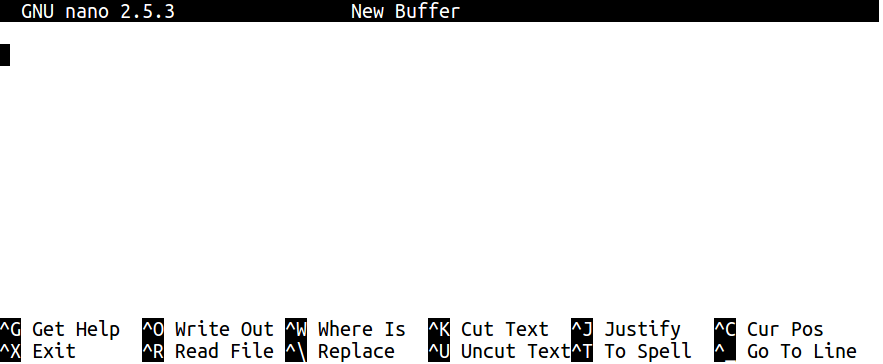
\includegraphics[width=\textwidth]{nano-blank}
\label{nano-b}
\end{figure} 
\quad\enskip\quad The options available in the nano text editor are listed along the bottom of the terminal window. The caret ($\wedge$) refers to the Ctrl button. The most important options are: \textbf{Ctrl-X} (close the program) and \textbf{Ctrl-O} (save file). Note these commands just need the Ctrl key and the letter (no shift key). \textbf{Ctrl-G} will display the help menu. Sometimes nano will prompt for user input (for example, what filename to save as). These prompts will appear just above the options list. For example, if a text file was edited, but not saved, nano will prompt the user to save the file upon closing. The file can be saved under a new name if needed. 

\quad Nano can take a bit of getting used to with regards to interactivity. Clicking on the text editor with the mouse does not move the cursor (blinking black object). Rather, the arrow keys or mouse wheel must be used to change the cursor's location.

\quad Other options include \textbf{Ctrl-R} (Read File), which allows the user to open a file from the current directory (or peruse the file structure - \textbf{Ctrl-T} or To Files). \textbf{Ctrl-W} (Where Is) will search the text file that is currently open for a string of characters. If it finds the string, it will highlight the start of that string with the cursor. The \textbf{Ctrl-J} (Justify) option only really applies if the terminal window has been resized. An example of where \textbf{Ctrl-J} can be used is shown in Figure \ref{nano-j}. To unjustify the text, use \textbf{Ctrl-U}. \textbf{Ctrl-C} (Cur Pos) shows where the cursor is currently in the file, including line number, column number, and character number. \textbf{Ctrl-K} and \textbf{Ctrl-U} can be used together to cut and paste (Uncut) text. \textbf{Ctrl-\textbackslash} can be used to find and replace strings of text. Nano will prompt yes or no for each matching instance that it finds.

\begin{figure}[H]
\centering
\caption{If the terminal is resized, some text may no longer show on one line. The justify option in nano should be used when the cursor is at the start of a paragraph (top left) to set the text to the same width as the terminal window. Lines that are too long for the window are indicated by a dollar sign (\$). Note that justifying text does not create line breaks.}
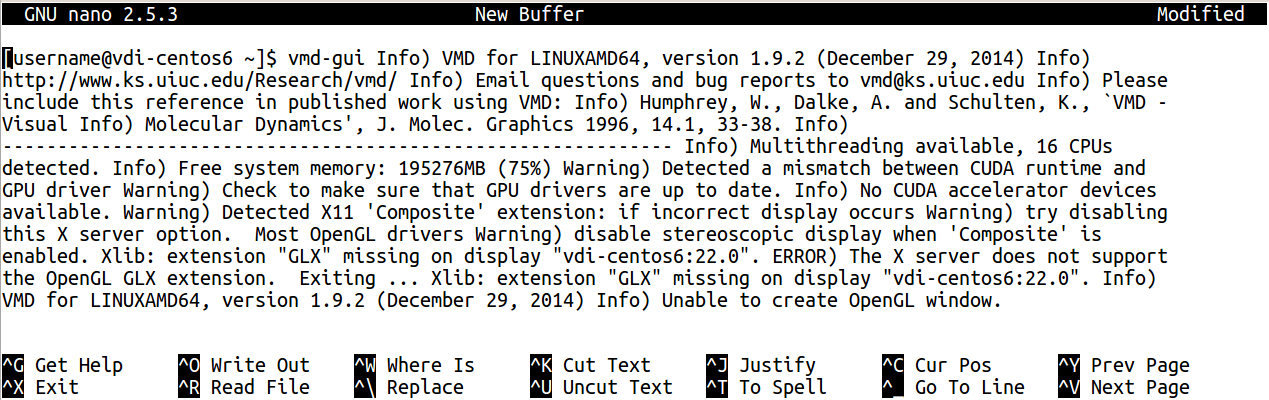
\includegraphics[width=\textwidth]{nano-justify-on}\\
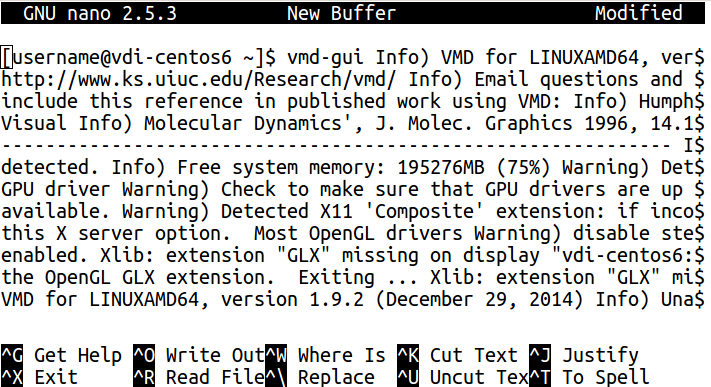
\includegraphics[scale=0.5]{nano-justify-off}
\label{nano-j}
\end{figure} 
  
\quad \textbf{Ctrl-T} starts the spell-checker in nano (Figure \ref{nano-s}), but this feature may not work by default. There is a line in the configuration file that can be enabled to add a spell-checker (shown below). However, to edit the \textit{/etc/nanorc} file, the user needs sudo access. If sudo access is not available, the user can make a file in the home directory (\textit{$\sim$/.nanorc}) and add commands to this file instead.

\begin{lstlisting}[numbers=none]
## Use this spelling checker instead of the internal one.  This option
## does not properly have a default value.
set speller "aspell -x -c"
\end{lstlisting}

\begin{figure}[H]
\centering
\caption{An example of the spell-checker in nano, after enabling the set speller line in the \textit{/etc/nanorc} file.}
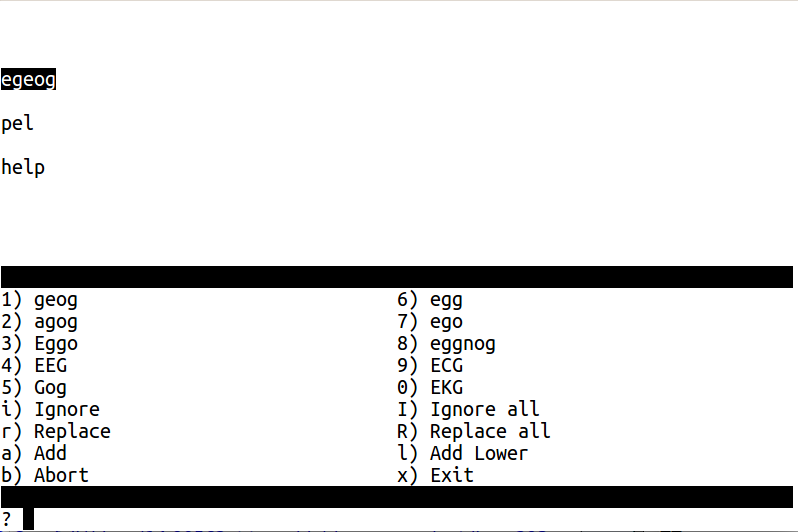
\includegraphics[width=\textwidth]{nano-spell}
\label{nano-s}
\end{figure}

\subsection{Other File Manipulation Options}

\quad\enskip\quad Sometimes, it is helpful to know what is in a file, but opening the file in nano is pointless. Instead, there is an option to use the command \textit{cat}. The \textit{cat} command is used for outputting the contents of a text file, or multiple text files (concatenation), to the terminal. For example, if there were two grocery lists, the cat command could show both:

\begin{lstlisting}[numbers=none]
username@oryx:~/Documents$ cat grocery1.txt grocery2.txt
Grocery List 1:
- beans
- cheese
- apple cider vinegar
- Smarties
- white bread
- BBQ sauce
- parchment paper
Grocery List 2:
- crayons
- butter
- chicken legs
- cheese
\end{lstlisting}
\quad\enskip\quad Another reason to use cat would be to make a new text file containing the contents of multiple text files. For example, to put both grocery lists in one file, use the right angle bracket ($>$, not hardware related) in the direction shown. The right angle bracket is the standard output.
\begin{lstlisting}[numbers=none]
username@oryx:~/Documents$ cat grocery1.txt grocery2.txt > groceries.txt
username@oryx:~/Documents$ cat groceries.txt 
Grocery List 1:
- beans
- cheese
- apple cider vinegar
- Smarties
- white bread
- BBQ sauce
- parchment paper
Grocery List 2:
- crayons
- butter
- chicken legs
- cheese
\end{lstlisting}
\quad\enskip\quad Before adding these two lists together, it might be helpful to see if there are any duplicates (i.e. cheese). For examples that are longer and less trivial, this command can really help to achieve an objective quickly. The \textit{diff} command will be helpful in comparing the contents two files. The argument \textit{-y} is used to show the outputs of both files side-by-side.
\begin{lstlisting}[numbers=none]
username@oryx:~/Documents$ diff -y grocery1.txt grocery2.txt 
Grocery List 1:              |  - Grocery List 2:
- beans                      |  - crayons
                             >  - butter
                             >  - chicken legs
- cheese                        - cheese
- apple cider vinegar        <
- Smarties                   <
- white bread                <
- BBQ sauce                  <
- parchment paper            <
\end{lstlisting}


\quad\enskip\quad Another helpful command is \textit{tail}. This command outputs the last 10 lines of a text file to the terminal. It is helpful when analysing a really large file. In the case of MD simulations, the programs often write data to a log file. At the end of the log file, the completion status of the program is shown (did the job finish successfully?). Rather than using cat to output the entire contents of the log file, tail can be used instead. This is what a successful job completion looks like for a NAMD job on Orca (Sharcnet):
\begin{lstlisting}[numbers=none]
[username@orc131 namd]$ tail step7.1_production.log 

WallClock: 42244.085938  CPUTime: 42244.085938  Memory: 934.199219 MB
[Partition 0][Node 0] End of program
--- SharcNET Job Epilogue ---
              job id: 5896362
         exit status: 0
        elapsed time: 11.7h / 13.0h (90 %)
      virtual memory: 6.3G / 1.8G (349 %)

Job completed successfully
\end{lstlisting}
And this is what a successful job completion looks like for a NAMD job on Guillimin (Calcul Qu\'{e}bec):
\begin{lstlisting}[numbers=none]
[username@lg-1r17-n02 nsep20025]$ tail step5.1_production.log 
FINISHED WRITING RESTART VELOCITIES
WRITING EXTENDED SYSTEM TO OUTPUT FILE AT STEP 500000
CLOSING EXTENDED SYSTEM TRAJECTORY FILE
WRITING COORDINATES TO OUTPUT FILE AT STEP 500000
CLOSING COORDINATE DCD FILE
WRITING VELOCITIES TO OUTPUT FILE AT STEP 500000
====================================================

WallClock: 16467.189453  CPUTime: 16467.189453  Memory: 259.929688 MB
End of program
\end{lstlisting}

\quad\enskip\quad Similar to cat, there are other commands for showing the contents of text files - \textit{less} and \textit{more}. These two commands work in a similar fashion, and show the full output of a file to the terminal.

\subsection{Compressed Files}

\quad Usually it is necessary to compress files (sometimes called adding to an archive) before they are sent to or received from a remote server. Compression reduces how much has to be sent over the network and therefore speeds up file transfer. Furthermore, if the transfer is interrupted before completion, the compressed archive can be deleted and resent more cleanly and easily. Compressed files are usually highlighted in red in the terminal, and can have extensions such as .tgz, .tar.gz, .zip, .gz, .7z, and .rar. Depending on the type of archive, a different command will be needed to interact with these files. 

\quad .tgz or .tar.gz can be easily worked with using linux machines. To create such an archive, use the following command: \textit{tar -czvf name-of-archive.tar.gz inputfile1.txt inputdirectory}, where c specifies creation of an archive. To decompress this archive, use the command: \textit{tar -xzvf name-of-archive.tar.gz}, where x specifies extraction of an archive. When creating or opening an archive, the -zvf arguments are: f for filename to work with, v for verbose (show files as they are being processed), and z means to work with a compressed archive. These commands retain the directory structure, and when archives are extracted, they will extract to the current directory.

\newpage

\section{Summary Table of Bash Commands}

\begin{table}[H]
\begin{changemargin}{-1.5cm}{-1.5cm}
\centering
\caption{A basic list of helpful terminal commands.}
{\renewcommand{\arraystretch}{1.4}% for the vertical padding
\begin{tabular}{|c|C{4.5cm}|C{9.5cm}|}
\hline
\textbf{Command} & \textbf{Description} & \textbf{Notes} \\
\hline
pwd & present working directory & get current path \\
ls & list directory contents & -a (hidden files), -h (human readable), -l (more details) \\
cd & change directory & cd <full path> or cd <subdirectory> \\
cp & copy & use -r (recursive) for copying directories \\
scp & secure copy & over ssh connection; use -r (recursive) for copying directories\\
mv & move & cut and paste file/directory to new location; can also rename file\\
exit & close a terminal & \\
ssh & secure shell & sign-in to remote host (ex: ssh username@system.ca) \\
logout & disconnect from remote host & \\
man & manual entry & followed by name of command, example: \textit{man ls}. can also try <command> $--$help \\
chmod & change mode & change permissions for file, example: \textit{chmod u+x file.txt} \\
chown & change owner & change who owns/created the file, may require sudo access. example: \textit{chown user:user file.txt} \\
export & set environment variable & example: \textit{export x=/home/user/Documents} \\
which & find location of executable & example: \textit{which ls} \\
grep & search & example: \textit{grep -i `query' file.txt}; -i means case insensitive \\
awk & file manipulation & example: \textit{awk `\{print \$2\}' file.txt}; \$2 refers to column 2 in file.txt \\


\hline
\end{tabular}
}
\label{big-table}
\end{changemargin}
\end{table}
\newpage
\begin{table}[H]
\begin{changemargin}{-1.5cm}{-1.5cm}
\centering
{\renewcommand{\arraystretch}{1.4}% for the vertical padding
\begin{tabular}{|c|C{4.5cm}|C{9.5cm}|}
\hline
\textbf{Command} & \textbf{Description} & \textbf{Notes} \\
\hline
echo & print to terminal & example: \textit{echo \$PATH}\\
nano & CLI text editor & open a blank file, or use \textit{nano /path/to/filename} \\
cat & concatenate files and print on the standard output & show output of text file, example: \textit{cat file.txt} \\
tail & print last ten lines of file & example: \textit{tail file.txt} \\
more | less & scan through files & \textit{more file.txt} or \textit{less file.txt} \\ 
diff & compare two files & determines if there are differences between two files given. use -y argument to show files side-by-side, with differences denoted by |. example: \textit{diff -y file1.txt file2.txt} \\
clear & clear terminal & puts prompt at the top of the terminal window; can still access previous output by scrolling upwards \\
reset | tput reset & clear terminal & prevents scrollback, refreshes terminal window while keeping set variables (local/environment) \\
module & interact with modules on HPC system & examples: \textit{module list, module avail, module load <modulename>, module unload <modulename>, module show <modulename>}. \\
rm & remove & PERMANENTLY REMOVES FILES, or remove directories (permanently) with -r. do not use unless absolutely sure you want to remove something - rm does not send files to a recycle bin!!! \\
tar -czvf & create compressed archive & example: \textit{tar -czvf archive-name.tar.gz directory-name} \\
tar -xzvf & extract compressed archive to current directory & example: \textit{tar -xzvf archive-name} \\

\hline
\end{tabular}
}
\end{changemargin}
\end{table}
\newpage

\section{Globus File Transfer}

\quad As an alternative to scp (secure copy) - see Section \ref{server}, Globus can be used to transfer files between servers and personal computers. The user will first need to register for a Globus account. Use the following link to their website: \url{https://www.globusid.org/login}.

\quad If you have yet to create a personal endpoint (and would like to transfer files between a home computer and a server), follow the instructions in Section \ref{globus-setup}. To transfer files between servers (or if you already have a personal endpoint), skip to Section \ref{useglobus}.

\subsection{Setting up Globus Connect Personal for the first time}\label{globus-setup}

\quad These instructions are only for those who wish to transfer files between their personal computers and a server. These instructions need only be followed once to setup an endpoint. 

\quad First, login to Globus: \url{https://www.globusid.org/login}. While still logged in, the user should generate a Setup Key from the website: \url{https://www.globus.org/app/endpoints/create-gcp}.

\begin{figure}[H]
\centering
\caption{To set-up a Globus endpoint on your personal computer, a name and Setup Key are required. The name should be an identifier for the computer to which the endpoint is connected.}
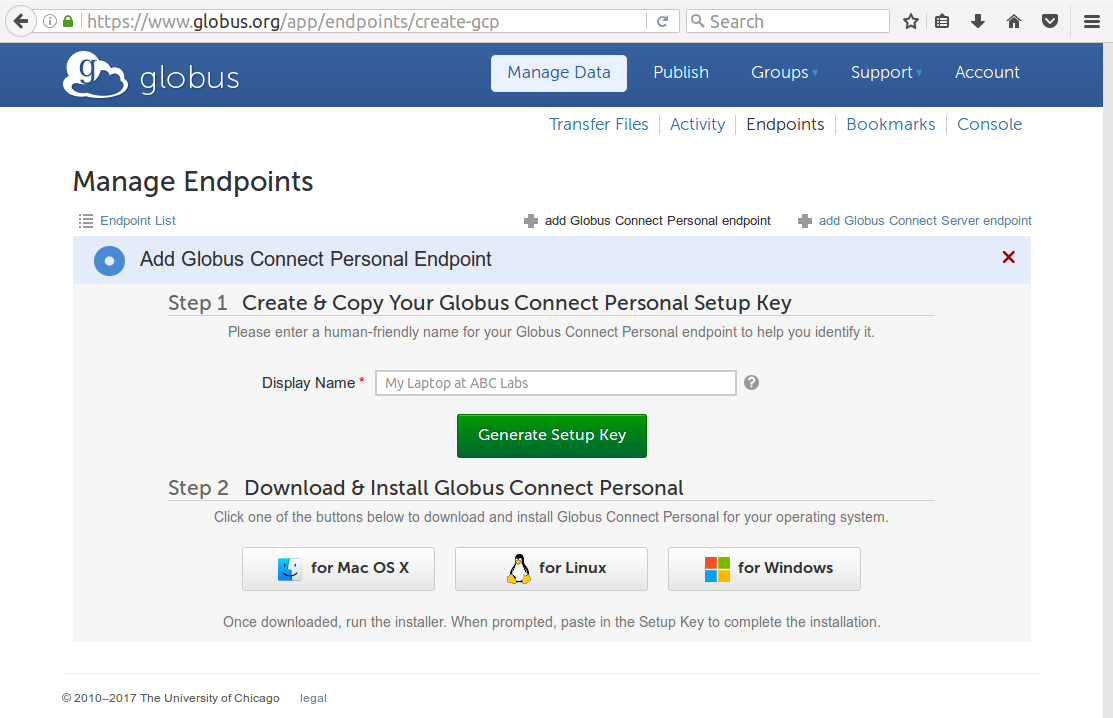
\includegraphics[width=\textwidth]{globus-1}
\label{globus-1}
\end{figure}

\quad The user should then download the Globus Connect Personal Package, either using the link shown in Figure \ref{globus-1} above, or by entering the following into a terminal:

\begin{lstlisting}[numbers=none]
user@localpc:~$ wget https://s3.amazonaws.com/connect.globusonline.org/linux/stable/globusconnectpersonal-latest.tgz
\end{lstlisting}

\quad The file should be extracted into an easily accessible directory on the local computer.

\begin{lstlisting}[numbers=none]
user@localpc:~$ tar -xzvf globusconnectpersonal-latest.tgz
\end{lstlisting}

\quad By extracting this archive, a directory should have appeared that looks similar to \textit{globusconnectpersonal-x.y.z}, where x.y.z is the version number that was downloaded. Go into that directory:

\begin{lstlisting}[numbers=none]
user@localpc:~$ cd globusconnectpersonal-x.y.z
\end{lstlisting}

\quad Then enter the setup key by running the globusconnectpersonal executable file. An example setup key is shown below. Replace this key with the one that was generated using your Globus account.

\begin{lstlisting}[numbers=none]
user@localpc:~/globusconnectpersonal-x.y.z$ ./globusconnectpersonal -setup 224532bb-8a4b-4d32-8995-e1fb442be98e
\end{lstlisting}

If everything goes smoothly, this should enable the globusconnectpersonal executable. The configuration files are saved in the home directory under /~/.globusonline/lta.

\quad This concludes the instructions for setting up Globus on a home computer. To transfer files using Globus, see Section \ref{useglobus}.

\subsection{Removing Globus Connect Personal}

\quad To remove Globus from a home computer, first kill any processes that Globus is running:
\begin{lstlisting}[numbers=none]
user@localpc:~$ killall gc-ctrl.py
\end{lstlisting}
Then remove the installation files from your home pc. You may get an error if these files have been moved or renamed.  For example, if they were downloaded to your home directory, cd to \$HOME and type:
\begin{lstlisting}[numbers=none]
user@localpc:~$ rm -r globusconnectpersonal-x.y.z globusconnectpersonal-latest.tgz
\end{lstlisting}
The last thing to do is remove the configuration files, which are stored in a hidden folder in your home directory:
\begin{lstlisting}[numbers=none]
user@localpc:~$ rm -r ~/.globusonline/
\end{lstlisting}

\subsection{Using Globus to transfer files}\label{useglobus}

\quad If transferring files using Globus Connect Personal (i.e. between your home pc and a server), first activate the endpoint. Go to where your Globus files are stored on your home computer, and run the globusconnect executable. Note: the tailing ampersand enables the use of the terminal while the Globus GUI is running.

\begin{lstlisting}[numbers=none]
user@localpc:~$ cd globusconnectpersonal-x.y.z
user@localpc:~/globusconnectpersonal-x.y.z$ ./globusconnect &
\end{lstlisting}

Then select \textit{Connect}. The Globus Online status should be green with a note that says "Connected".

\begin{figure}[H]
\centering
\caption{Before transferring files between a home computer and a server, the globus endpoint must be activated from the home computer.}
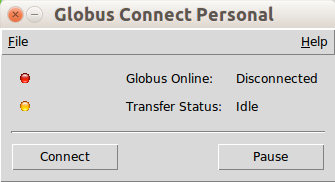
\includegraphics[width=.46\textwidth]{globus-off} 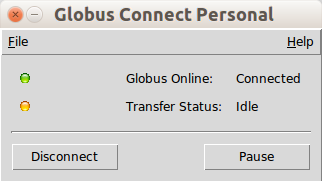
\includegraphics[width=.45\textwidth]{globus-on}
\label{globus-status}
\end{figure}

\quad To transfer files, logon to the Globus website \url{https://www.globusid.org/login} and go to transfer files \url{https://www.globus.org/app/transfer}. 

\begin{figure}[H]
\centering
\caption{This is the main screen for transferring files using Globus.}
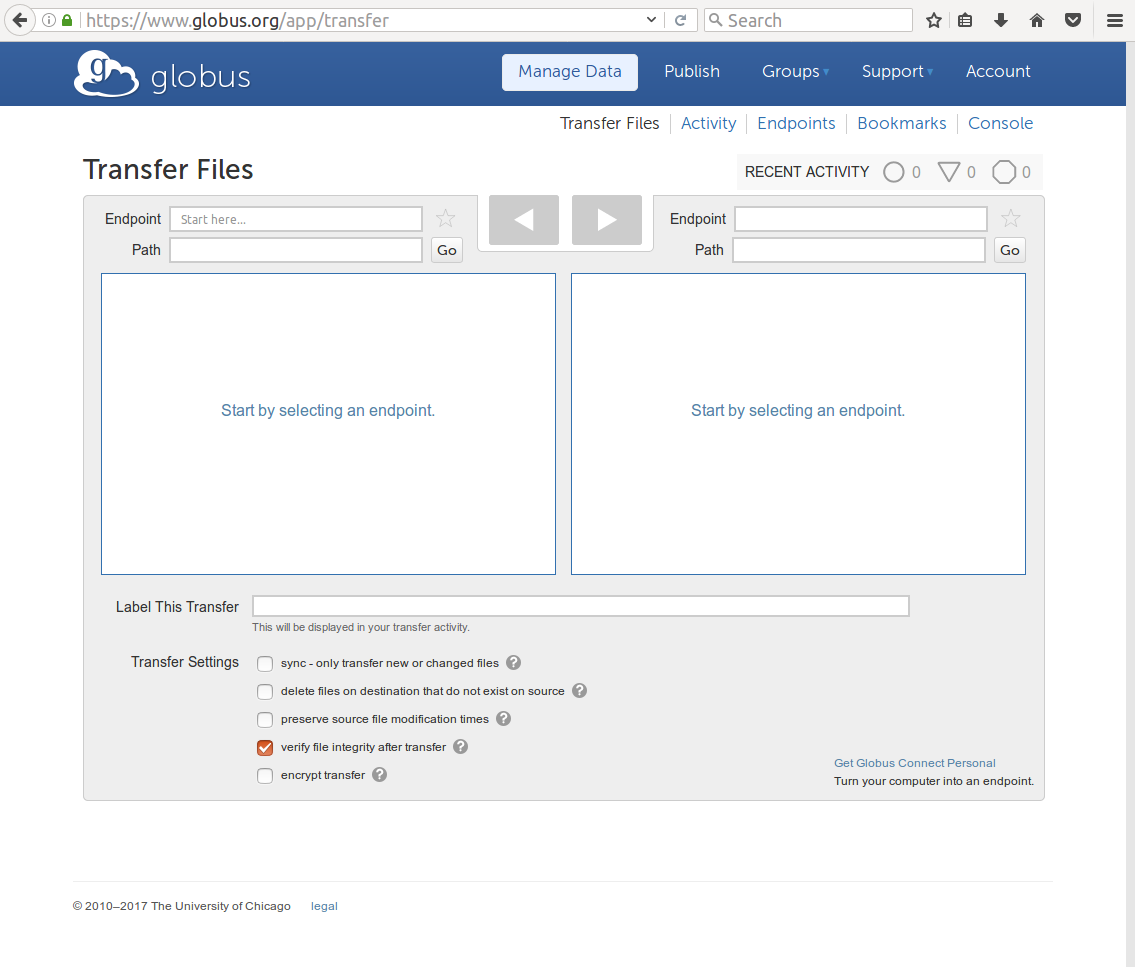
\includegraphics[width=\textwidth]{globus-transfer}
\label{globus-trsf}
\end{figure}

\quad Then, select the white box on either the left or right side that says \textit{Endpoint}. If you want to select your home computer as an endpoint, select \textit{Administered by Me} and choose the name that was chosen when Globus was set-up.

\begin{figure}[H]
\centering
\caption{Any endpoints that have been set-up by your account on a home computer will be listed under the "Administered by Me" tab.}
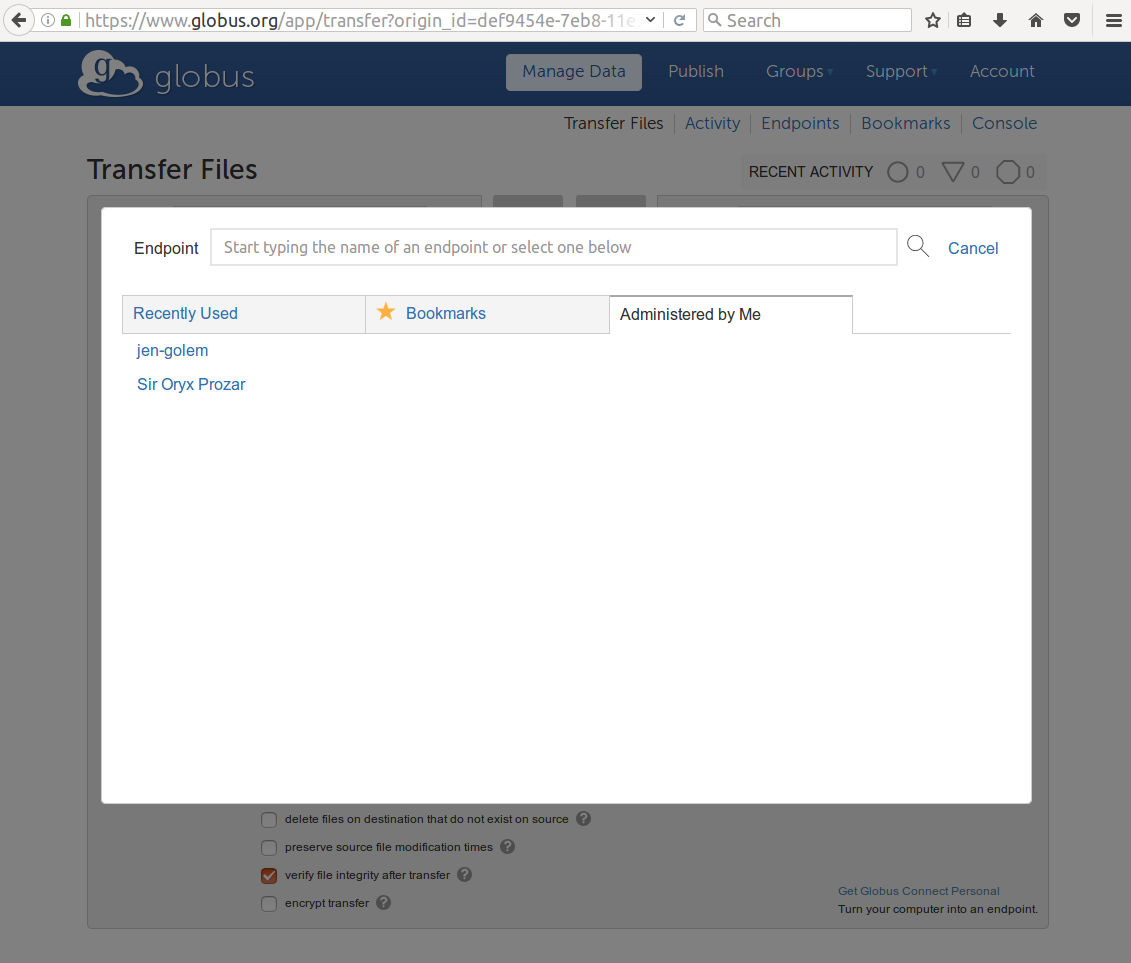
\includegraphics[width=\textwidth]{globus-select}
\label{globus-sel}
\end{figure}

\quad To select a server as an endpoint, enter the name of the server into the top white box shown in Figure \ref{globus-sel} that says \textit{Start typing the name of an endpoint or select one below}. Common server names are:

\begin{table}[H]
\centering
{\renewcommand{\arraystretch}{1.2}% for the vertical padding
\begin{tabular}{c|c}
Server Name & Endpoint Name \\
\hline
Graham (Compute Canada) & computecanada\#graham-dtn \\
Orca (Sharcnet) & computecanada\#sharcnet-dtn1 \\
Briaree (Calcul Qu\'{e}bec) & computecanada\#briaree \\
Guillimin (Calcul Qu\'{e}bec) & computecanada\#guillimin
\end{tabular}
}
\end{table}

It should be noted that since most of the Sharcnet systems are linked under a common storage space, the endpoint would be the same for other Sharcnet systems (for example: Monk) as for Orca. When you select these endpoints, you will be required to sign in using your corresponding credentials. 

\quad Another consideration is the directory from which you wish to transfer files. The default directory that is opened is the home directory (/$\sim$/); however, most jobs are stored in the project or scratch directories. You will need to enter the corresponding directory into the white box labelled \textit{Path} - see Figure \ref{globus-trsf}. For example, to access the scratch directory in Graham, enter /scratch/user (where user is replaced by the real username) into the Path box.

\subsection{How to add a new path to Globus}

\quad By default, Globus Connect Personal only has access to your home directory (/$\sim$/). If you have an external hard drive or USB device, these are not likely to be mounted in the home directory. Therefore, you must give Globus permission to access them. Usually, such external drives are stored in Linux machines under the /media/username directory. You can add this path (to enable access to all mountable media) or a specific path to Globus by opening the Globus Connect Personal GUI window (Figure \ref{globus-status}) and selecting File $\rightarrow$ Preferences. A new window should open called \textit{Access Path Configuration}, as shown in Figure \ref{globus-add}.

\begin{figure}[H]
\centering
\caption{An example of an external hard drive whose path was added to the list of writable directories, as accessible from the Globus website.}
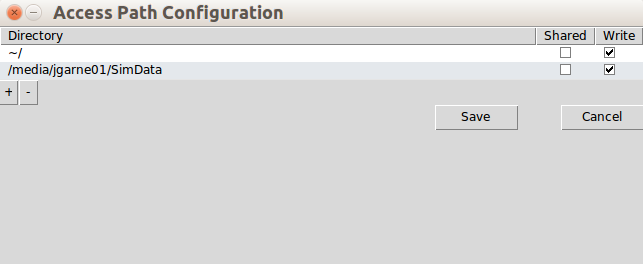
\includegraphics[width=.8\textwidth]{globus-addusb}
\label{globus-add}
\end{figure}

\quad Select the plus (+) button on the left, type the path to your files, and select \textbf{Save}. If you want to add files to this new path from elsewhere (i.e. from a server), make sure to make the directory writable by ticking the \textbf{Write} box beside the corresponding directory. You should now be able to access the contents of this directory from the Globus website.

\section{Compute Canada - Graham}\label{CompC}
\quad\enskip\quad This section will be devoted to the new system called Graham. It uses a scheduler called slurm \url{https://slurm.schedmd.com/}. The help email for this system is: \textit{support@computecanada.ca}. 

\subsection{Logging On and Off}

\quad To access Graham from a terminal, use the \textit{ssh} command and your Compute Canada credentials (note these credentials are not the same as the Sharcnet or Calcul Qu\'{e}bec login credentials). When you are finished using a system through ssh, the command is \textit{logout}. This command will return you to the local system.

\begin{lstlisting}[numbers=none]
username@localpc:~$ ssh username@graham.computecanada.ca
username@graham.computecanada.ca's password: 

Welcome to the ComputeCanada/SHARCNET cluster Graham.

Please refer to the following page:
https://docs.computecanada.ca/wiki/Graham

Email support@computecanada.ca for assistance.

***

[username@gra-login3 ~]$ logout 
Connection to graham.computecanada.ca closed.
username@localpc:~$ 

\end{lstlisting}

\quad Provided that users have a single project on Compute Canada, it is recommended that the $\sim$/.bashrc file be altered (using \textbf{nano} or some other basic text editor). The addition (shown below) fulfills the requirement that all jobs specify the group name, without having to write in the account for every job submission.

\begin{lstlisting}[numbers=none]
export SLURM_ACCOUNT=def-someuser
export SBATCH_ACCOUNT=$SLURM_ACCOUNT
export SALLOC_ACCOUNT=$SLURM_ACCOUNT 
\end{lstlisting}

Where someuser should be replaced by the group name. The group name can be found by logging onto the Compute Canada website and listing the project details. Alternatively, you can determine the group name by using the \textit{groups} command while logged on to Graham.



\subsection{Submitting Basic Jobs}
\quad\enskip\quad To submit a job to Graham, the command \textit{sbatch} is used. More information can be found on the Compute Canada help wiki: \url{https://docs.computecanada.ca/wiki/Running_jobs}.

\quad Some basic arguments for the sbatch command include:
\begin{lstlisting}[numbers=none, basicstyle=\normalsize]
-t # time to complete the job
-J # job name
--mem=4G # (for example) for requesting memory (G=gigabytes, M=megabytes, K=kilobytes, etc., where the default unit is megabytes) 
-N # number of nodes
-n # number of tasks (which can be thought of as number of CPUs) 
--gres=gpu:2 # (for example) for generic resource, such as GPU
-o # output file name
-e # error output file name (by default the error file is included in the output file)
\end{lstlisting}
 A full list of arguments can be found here: \url{https://slurm.schedmd.com/sbatch.html}. Note that most arguments have an explicit form (example $--$time=00:60:00) or a short form (example $-$t 00:60:00). 
 
\quad For example, to submit a script called my-script.py to run on Graham for 20 minutes and writing to a file called output.txt, the command would be: 
\begin{lstlisting}[numbers=none, basicstyle=\normalsize]
sbatch -t 00:20:00 -o output.txt ./my-script.py
\end{lstlisting}

\quad If the user has not specified the job name as an environment variable in the $\sim$/.bashrc, it will be necessary to add the account argument with every submission.

\begin{lstlisting}[numbers=none, basicstyle=\normalsize]
sbatch -t 00:20:00 -o output.txt --account=def-someuser ./my-script.py
\end{lstlisting}

\quad As with other servers, some jobs may require loading modules prior to submission. The same commands can be used on Graham as with other servers (i.e. \textit{module (un)load}, \textit{module list}, and \textit{module avail} all work). For example, the default version of python on Graham is python2.7. To load another version of python, use:

\begin{lstlisting}[numbers=none]
[username@gra-login3 ~]$ module load python/3.5.2
[username@gra-login3 ~]$ module list

Currently Loaded Modules:
  1) nixpkgs/16.09 (S)   4) ifort/.2016.4.258 (H)  7) openmpi/2.1.1 (m)
  2) icc/.2016.4.258 (H) 5) intel/2016.4    (t)    8) StdEnv/2016.4 (S)
  3) gcccore/.5.4.0  (H) 6) imkl/11.3.4.258 (math) 9) python/3.5.2  (t)

\end{lstlisting}

\subsection{Checking Job Status}

\quad To see what jobs are currently running, use the \textit{squeue} command. You can also add the argument \textit{-u \$USER} to only see jobs for a given user. For example:

\begin{lstlisting}[numbers=none, basicstyle=\tiny]
[username@gra-login2 ~]$ squeue -u $USER
   JOBID  USER  ACCOUNT  NAME  ST START_TIME TIME_LEFT NODES CPUS   GRES MIN_MEM NODELIST (REASON) 
  433759 user  group    job1a  PD N/A          2:00:00  1      32  gpu:2  2G           (Priority) 
  433765 user  group    job1b  PD N/A          2:00:00  1      32  gpu:2  2G         (Dependency) 
  433766 user  group    jobA   PD N/A          0:30:00  1      32  gpu:1  1G          (Resources) 
\end{lstlisting} 

\quad Here we have three jobs listed in the queue. The "REASON" column explains the state (ST) of the job (where PD is pending, R is running). Priority means that other users have higher priority than your group and are in line next to use resources. Dependency means that another job has to start somehow before its dependent job can run (i.e. job1a must finish before job1b can run). Resources means that the scheduler is waiting on resources in use before the job can start. 

\subsection{Cancelling a Job}

\quad Use \textit{scancel jobid} to cancel a job, where jobid should be replaced by the number for the job you want to cancel. Similarly, to cancel all jobs for a user, use \textit{scancel -u \$USER}. To cancel all pending jobs, use \textit{scancel -u \$USER -t PENDING}. For more information on the scancel command, follow this link \url{https://slurm.schedmd.com/scancel.html}.

\subsection{Submitting a job using a script}

\quad When a user has a job that is more complicated, usually they will write a script to submit that job. A script can be generated in a basic text editor on Graham. Scripts can also be written on the local system and subsequently uploaded to Graham. For information on how to transfer files between th

\newpage

\section{Calcul Qu\'{e}bec Systems}\label{CalcQ}

\quad Systems currently in use:
\begin{itemize}
\item Briaree
\item Guillimin
\end{itemize}
\quad\enskip\quad Another system on Calcul Qu\'{e}bec is Helios - a GPU system. It may be used for future work if needed. Information with regards to submitting jobs on Calcul Qu\'{e}bec systems can be found here: \url{https://wiki.calculquebec.ca/w/Ex%C3%A9cuter_une_t%C3%A2che/en#tab=tab4}. 


\subsection{Briar\'{e}e}

\subsubsection{Briar\'{e}e Resources}

\quad Briar\'{e}e is a CPU system on Calcul Qu\'{e}bec. It has a total of 672 nodes, with 12 cores per node. The RAM available depends on the node; nodes can have 24, 48, or 96GB of RAM, or 2, 4, or 8GB per core respectively.

\quad Jobs on Briar\'{e}e can spend a maximum of 7 days running (not including time spent in the queue). There is a default limit of 4 nodes per job, meaning that the maximum number of cores that can be requested is 48. To get access to more nodes, users must provide scaling figures (i.e. benchmarking numbers) to the support staff at Calcul Qu\'{e}bec. These figures must display that the code will benefit from more resources (scales well) when using the appropriate software. The support staff for Briar\'{e}e can be emailed at: briaree@calculquebec.ca.

\quad The storage space on Briar\'{e}e is divided into two main sections: home (located at /RQusagers/username) and scratch (located at /RQexec/username). The home space is backed up, and the scratch space is not backed up. These spaces do not have a specified quota, but the limits should be similar to those for Guillimin (10GB home, 1TB scratch). The scratch space is not cleared for Briar\'{e}e as it is for Guillimin, but there is no designated project space for Briar\'{e}e. The storage space used by both Briar\'{e}e and Guillimin is called GPFS, which is a high-performance storage space that allows for good throughput for parallel jobs.

\quad Module information for Briar\'{e}e can be found at this website: \url{https://wiki.calculquebec.ca/w/Modules_disponibles_sur_Briar%C3%A9e?setlang=en}

\subsubsection{MWE for Briar\'{e}e Submission Script}
\quad To run this script, open a terminal and type: \textit{bash scriptname.bash}. 
\begin{lstlisting}
#!/bin/bash
#PBS -r n
#PBS -A nmf-334-aa
#PBS -N job-name
#PBS -l mem=2GB
#PBS -l nodes=2:ppn=12
#PBS -l walltime=01:00:00
#PBS -j oe
module purge
module load NAMD/2.9
module load python/2.7.1
cd $PBS_O_WORKDIR
mpiexec -n 24 namd2 input-file.inp > output-file.log
\end{lstlisting}

\quad By line number, here is an explanation for this script:

\begin{enumerate}
\item execute this script using bash commands
\item job should not be automatically restarted if there are issues
\item RAP ID for the project
\item job name (should be short)
\item how much RAM to allocate for the job
\item how many nodes and processors per node (ppn) to allocate for the job
\item how long the job will take to complete (set for 1 hour)
\item join the output and error files to one file
\item remove all currently loaded modules
\item load the NAMD module
\item load the python module
\item change directory to the working directory
\item run the input-file.inp using the namd2 exectuable, with 24 cores for the job (2x12), on the mpiexec queue, and write the ouput to the output-file.log file
\end{enumerate}

\subsection{Guillimin}
\subsubsection{Guillimin Resources}

\quad Guillimin is a CPU system on Calcul Qu\'{e}bec. It has a total of 1582 nodes, where 1200 of these nodes have 12 cores per node and the remaining 382 nodes have 16 cores per node. The RAM available depends on the node; 12-core nodes can have 24, 36, or 72GB of RAM, or 2, 3, or 6GB per core respectively. The 16-core nodes can have 64, 128, 256, 384, 512, or 1024GB of RAM, or 4, 8, 16, 24, 32, or 64GB per core respectively.

\quad Jobs on Guillimin can spend a maximum of 30 days running (not including time spent in the queue). The support staff for Guillimin can be emailed at: guillimin@calculquebec.ca.

\quad The file structure for Guillimin is unique compared to other Calcul Qu\'{e}bec systems. The user has access to two main locations for their files: the home directory (located at /home/username) and the project directory (located at /gs/project/nmf-334-aa, where nmf-334-aa is the project or RAP ID). There is also the scratch directory (located at /gs/scratch/username) that can be used to store temporary files. Files stored on the scratch directory will be deleted if they are not updated after 45 days. The cleanup occurs on the 15th day of each month, with users being warned on the 8th day of each month if there are files that are going to be deleted. More information about file storage on Guillimin can be found on this website: \url{http://www.hpc.mcgill.ca/index.php/starthere/81-doc-pages/87-disk-space}.

\quad To determine how much disk space is being used on Guillimin, the commands \textit{myquota} and \textit{prquota} can be used for the home/scratch and project spaces respectively. The home directory is backed up on a daily basis, and has a quota size of 10GB. This location is used for important files that are used regularly (such as submission scripts). The project space is not backed up, but can be used to store more files. It has a quota of 1TB across all project members. Lastly, the scratch space has a quota of 1TB per user, and it should be used to store temporary files and/or files that are being run.

\quad Module information for Guillimin can be found at this website: \url{https://wiki.calculquebec.ca/w/Modules_disponibles_sur_Guillimin?setlang=en}

\subsection{MWE for Guillimin Submission Script}

\begin{lstlisting}
#!/bin/bash
#PBS -A nmf-334-aa
#PBS -l walltime=10:00:00
#PBS -l nodes=3:ppn=12
#PBS -l pmem=7700m
module purge
module load openmpi/1.6.3-gcc
module load NAMD/2.9-openmpi-gcc
module load python/2.7.9
cd $PBS_O_WORKDIR
mpiexec -n 36 namd2 input-file.inp > output-file.log
\end{lstlisting}

\quad Note that assigning RAM for Guillimin jobs is slightly different than for Briar\'{e}e. Otherwise, these are the minimum number of instructions that should be given for a job submission. The -n argument specifies to use 36 cores for the job (3x12).

\section{Sharcnet Systems}\label{Sharc}

\quad Systems currently in use:
\begin{itemize}
\item Monk
\item Orca
\item Saw
\end{itemize}

\quad Getting help for Sharcnet systems involves submitting a ticket, and there is a unified help email (unlike Calcul Qu\'{e}bec, which has emails per system). Contact: help@sharcnet.ca. Sharcnet also has regular webinars that can be accessed via VidyoDesktop. These webinars are also uploaded to their youtube channel. The webinars are typically 1 hour long and run on Wednesdays at noon (12pm). They cover a variety of computing topics.

\subsection{Sharcnet File Storage}
\quad For the most part, Sharcnet has a unified storage space across the systems mentioned in this document: Monk, Orca, Saw, and vdi-centos6. This means that any files generated by these systems will be accessible by the other systems. The details for the Sharcnet file storage can be found on this webpage: \url{https://www.sharcnet.ca/my/systems/storage}. 

\quad The home storage space (located at /home/username) has a quota of 10GB per user and is backed up. It should be used for important files such as source code, scripts, parameters, etc. The user cannot exeed the quota, which means that jobs will not be able to write data to the home space past 10GB. 

\quad The work directory (located at /work/username) has a quota of 1TB, but it is not backed-up. It should be used for large files. The scratch directory (located at /scratch/username) can be used for large file storage (no quota), but files must be deleted or moved from this space, as files will be removed after 62 days. 

\quad The freeezer directory (located at /freezer/username for orca login nodes and /global/freezer/username for saw login nodes) has a quota of 2TB; files stored here have a lifetime of 2 years. This space can only be accessed from login nodes (for example, you can only access the freezer directory from login not after ssh to a development node).

\begin{lstlisting}[numbers=none]
[username@saw-login1 ~]$ cd /global/freezer/username
[username@saw-login1 username]$ ssh saw-dev1
[username@saw331 ~]$ cd /global/freezer/username
-bash: cd: /global/freezer/username: No such file or directory
\end{lstlisting}
\quad The command \textit{quota} will show the file usage for the work and home directories on Sharcnet. Alternatively, login to the Sharcnet web portal - \url{https://www.sharcnet.ca/my/security/login} - and scroll down to \textbf{Disk Usage}, which will show a plot of the files stored by age in the home and work directories. If the user exceeds their quota for either the work or freezer directories, the user has a 3-day grace period to reduce their file count. After the grace period, if the user has not reduced their file count, he/she will no longer be able to submit jobs on Sharcnet. Quotas are updated at approximately midnight each day, but this update depends on the disk usage and the system.

\subsection{Monk}

\subsubsection{Monk Resources}
\quad Monk is a GPU system on Sharcnet. It has a total of 54 nodes, with 8 cores, 2 GPUs, and 48GB of RAM per node. This system should only be used for jobs that can make use of GPU acceleration. It is tied-in to the file-system shared by Orca, Saw, and other Sharcnet systems.

\subsection{Orca}

\subsubsection{Orca Resources}

\quad Orca is a CPU system on Sharcnet. It has a total of 392 nodes, split into 4 groups. Group 1 (nodes 1-320) has 24 cores and 32GB RAM per node. Group 2 (nodes 321-360) has 16 cores and 32GB RAM per node. Group 3 (nodes 361-388) has 16 cores and 64GB RAM per node. Lastly, group 4 (nodes 389-392) has 16 cores and 128GB RAM per node. Orca has 4 development nodes: orc-dev1, orc-dev2, orc-dev3, and orc-dev4. These development nodes should be accessed after logging in to the system (\textit{ssh orc-dev1}). The login nodes are not supposed to support heavy CPU usage, and are designed as a stable access point to the system. Code can be run from these development nodes directly (without submitting to the queue) for testing purposes. These sorts of programs can be run for up to 3 CPU days (which is not equal to 3 days). 

\subsection{Saw}

\subsubsection{Saw Resources}

\subsection{Sharcnet Visualisation Systems}\label{visual}

\quad Some systems on Sharcnet are used for visualisation purposes - that is, the user can use graphics programs and is not restricted to the command-line interface. The documentation for these systems can be found here: \url{https://www.sharcnet.ca/help/index.php/Remote_Graphical_Connections}. One such system is called centos6-vdi. The documentation for this system can be found here: \url{https://www.sharcnet.ca/my/systems/show/104}. 

\subsubsection{Accessing vdi-centos6}

\quad This system can be accessed from any computer using a web-browser. Open this url: \url{https://www.sharcnet.ca/my/systems/show/104} and select the \textbf{Web graphical desktop} link - see Figure \ref{vdi-link}.

\begin{figure}[H]
\centering
\caption{The vdi-centos6 system on Sharcnet can be accessed using a web-browser, such as Chrome or Firefox. The link is circled in the figure below.}
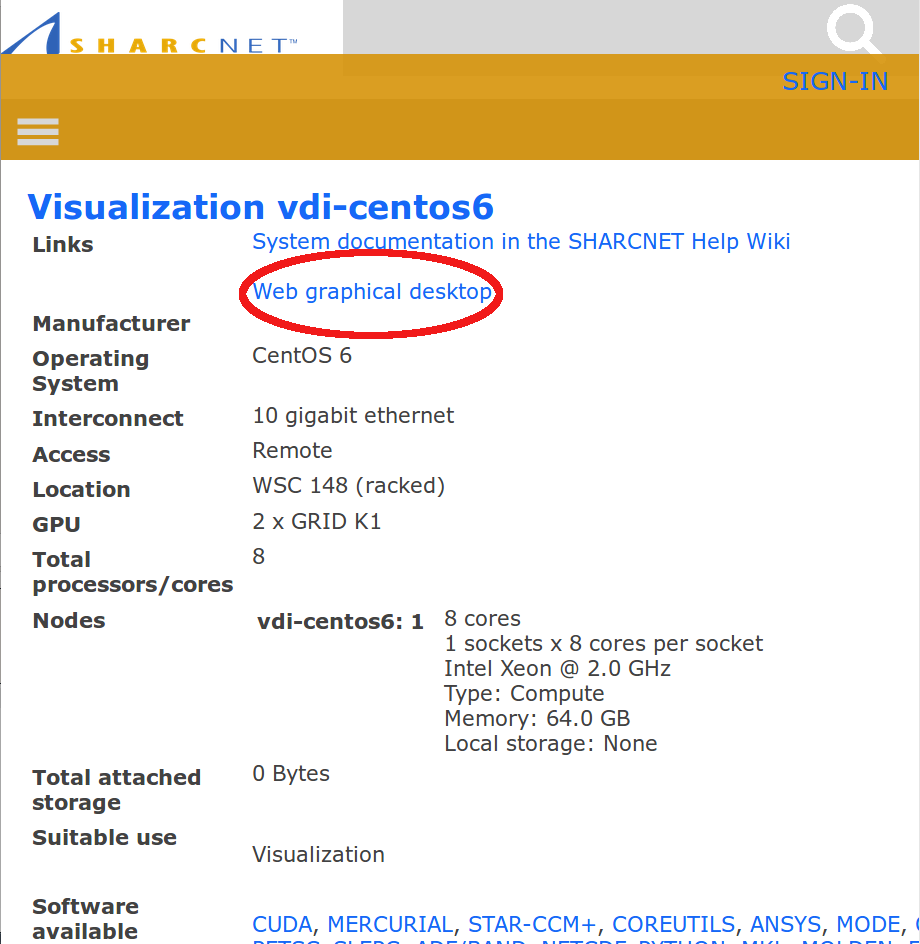
\includegraphics[width=.7\textwidth]{vdi-link}
\label{vdi-link}
\end{figure}

\quad Another way to access vdi-centos6 is by using a VNC client. For Ubuntu, the recommended client is called gvncviewer. To install, configure, and use the gvncviewer program, follow these instructions: 
\begin{lstlisting}
apt-get install gvncviewer
mkdir -p ~/.pki/CA
ln -s /etc/ssl/certs/ca-certificates.crt ~/.pki/CA/cacert.pem
gvncviewer vdi-centos6.user.sharcnet.ca
\end{lstlisting}
The user only has to install (line 1) and configure (lines 2 and 3) the gvncviewer once. If these instructions have been used previously, the last command (line 4) is all that is needed. Note that \textit{user} here does NOT mean username. See Figure \ref{vdi-login} for an example of the VNC client.

\begin{figure}[H]
\centering
\caption{The vdi-centos6 system on Sharcnet can be accessed on Ubuntu using a VNC client such as gvncviewer. When the command \textit{gvncviewer vdi-centos6.user.sharcnet.ca} is used, the user will be prompted for their Sharcnet username and password.}
\includegraphics[width=\textwidth]{vdi-login}
\label{vdi-login}
\end{figure}

\quad To logout from vdi-centos6, simply close the web-browser or (if using gvncviewer) close the gvncviewer window. To close a terminal that has been opened on this system, the command is \textit{exit} rather than \textit{logout}. The \textit{exit} command also applies for closing terminals open on the user's home computer.

\subsubsection{Graphical VMD via vdi-centos6}

\quad This system is helpful for simulation work. It enbales the user to open, view, and analyse simulation data stored on the global filesystem of Sharcnet using VMD, without downloading all of the files to a home computer. To use the graphical version of VMD

\begin{figure}[H]
\centering
\caption{The vdi-centos6 system can be used to open a graphical version of VMD. The user first needs to load the \textit{vmd/tachyon/1.9.2} module. Note that the version number may change over time, and so use \textit{module avail} to see the current version on the system.}
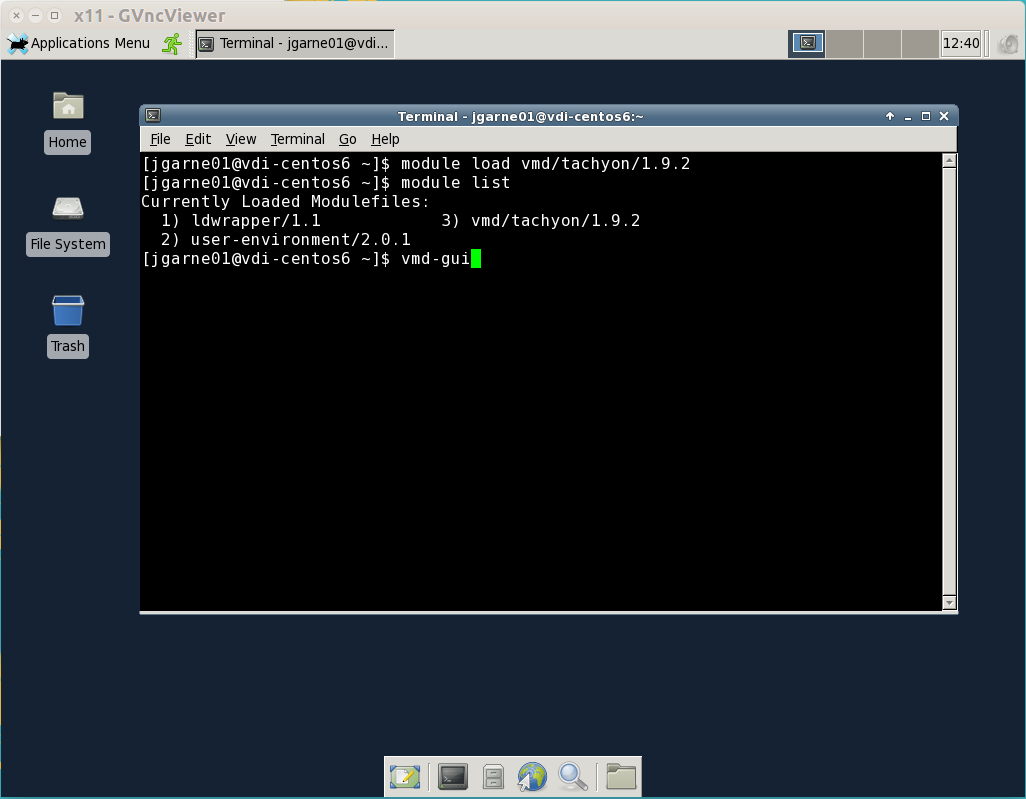
\includegraphics[width=\textwidth]{vdi-load-vmd}
\label{vdi-load-vmd}
\end{figure}

\begin{figure}[H]
\centering
\caption{An example of the graphical version of VMD opened using the vdi-centos6 system.}
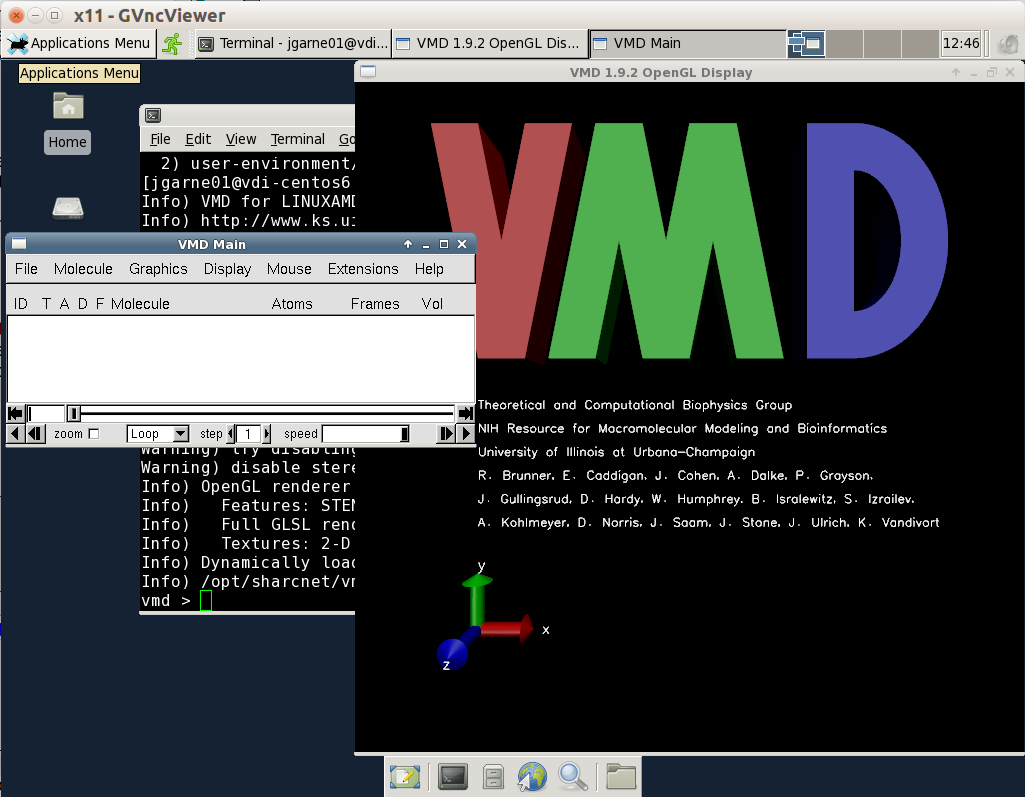
\includegraphics[width=\textwidth]{vdi-vmd-gui}
\label{vdi-vmd-gui}
\end{figure}

\section{Abbreviations}
\centering

\begin{tabular}{c|c}
Abbreviation & Full Name \\
\hline
RAM & Random Access Memory \\
MWE & Minimum Working Example \\
HPC & High Performance Computing \\
VNC & Virtual Network Computing \\
VMD & Visual Molecular Dynamics (Program) \\
GB & gigabyte ($10^9$ bytes) \\
MB & megabyte ($10^6$ bytes) \\
KB & kilobyte ($10^3$ bytes) \\
ppn & processors per node (for Calcul Qu\'{e}bec) \\
\end{tabular}

\end{document}